\documentclass{article}
\usepackage{amsmath}
\usepackage{amssymb}
\usepackage{graphicx}
\usepackage{hyperref}
\usepackage[version=4]{mhchem}

\title{Problem 6}
\date{}

\begin{document}
\maketitle

\section*{Problem}
In \(\triangle A B C, A C>A B . D\) is on \(A C\) such that \(C D=A B . E\) and \(F\) are the midpoints of \(A D, B C\), respectively. Connect \(E F\) and extend it to meet the extension of \(B A\) at \(G\). Prove: \(A E=A G\).\\
\centering
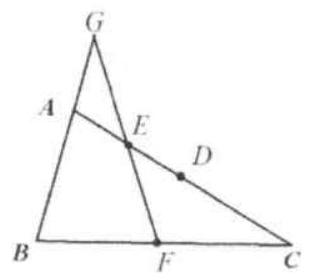
\includegraphics[width=\textwidth]{images/problem_image_1.jpg}

\section*{Solution}
Take \(H\), the midpoint of \(B D\).\\
Connect EH, FH.\\
Since \(E\) and \(H\) are midpoints of \(A D, B D\), respectively, by Theorem 2.1, \(E H / /\)

\[
A B, E H=\frac{1}{2} A B
\]

Since \(F\) and \(H\) are midpoints of \(B C, B D\), respectively, by\\
Theorem 2.1, \(H F / / C D, H F=\frac{1}{2} D C\)\\
\centering
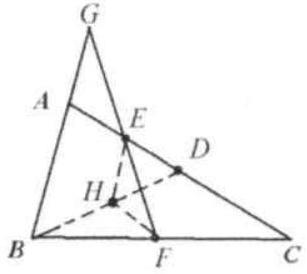
\includegraphics[width=\textwidth]{images/reasoning_image_1.jpg}

Since \(C D=A B, E H=H F . \angle H E F=\angle H F E\).\\
Since \(K F / / A C, \angle A E G=\angle K F G\) or \(\angle A E G=\angle H F E\).\\
Since \(E H / / G K, \angle G=\angle H E F\)\\
Thus \(\angle G=\angle A E G, A E=A G\).

\end{document}
